\section*{Глава 2. Проектирование веб-приложения}
\addcontentsline{toc}{section}{Глава 2. Проектирование веб-приложения}
\stepcounter{section}

\subsection{Анализ целевой аудитории}

Эффективность проектирования веб-приложения для управления и мониторинга CI/CD-пайплайнов напрямую зависит от детального понимания потребностей будущих пользователей. В условиях командной разработки программного обеспечения с конвейерами непрерывной интеграции взаимодействуют специалисты с различными зонами ответственности.

На основе специфики предметной области выделены три ключевые группы пользователей:
\begin{enumerate}
    \item DevOps-инженеры и системные администраторы. Специалисты отвечают за стабильность сборочной инфраструктуры, конфигурацию раннеров и доступность внешних платформ. Их ключевой интерес заключается в сквозном контроле работоспособности конвейеров, обнаружении зависших задач, анализе времени прохождения стадий и устранении инфраструктурных сбоев.
    \item Разработчики программного обеспечения (Frontend, Backend, Fullstack). Основные потребители сервиса. Для них критически важно быстро получать обратную связь о статусе прохождения юнит-тестов, линтеров и сборок после отправки изменений в Git. В случае падения сборки разработчику необходим моментальный доступ к логам ошибки и возможность повторного перезапуска задачи в один клик.
    \item Технические руководители и тимлиды (Team Lead, Tech Lead). Пользователи заинтересованы в высокоуровневой аналитике: общем проценте успешных сборок (Success Rate), частоте релизов, выявлении нестабильных тестов и контроле готовности релизных веток.
\end{enumerate}

Для формализации требований сформированы репрезентативные профили целевых пользователей (User Personas), представленные в таблице~\ref{tab:user_personas}.

\begin{table}[H]
    \centering
    \caption{Профили целевых пользователей (User Personas)}
    \label{tab:user_personas}
    \small
    \resizebox{\textwidth}{!}{%
    \begin{tabular}{|p{3cm}|p{3.8cm}|p{4.2cm}|p{3.8cm}|}
        \hline
        \textbf{Персона} & \textbf{Контекст деятельности} & \textbf{Боли и проблемы} & \textbf{Ожидания от системы} \\ \hline
        Алексей, 28 лет, DevOps-инженер & Сопровождает 15 микросервисов, распределенных между GitHub и GitLab & Вынужден переключаться между десятком вкладок; сложно отслеживать зависшие сборки & Единая панель статусов; фильтрация по статусам; оперативные уведомления \\ \hline
        Илья, 23 года, Backend-разработчик & Пишет код, часто делает push в feature-ветки, ждет результатов тестов & Долго ищет упавший шаг в громоздких интерфейсах; сложный путь до кнопки «Retry» & Моментальное отображение статуса коммита; лог ошибки на одном экране; быстрый перезапуск \\ \hline
        Марина, 34 года, Team Lead & Контролирует поставку релизов и метрики качества в спринтах & Отсутствие наглядной сводки по стабильности репозиториев; разрозненные отчеты & Обзорный дашборд; графики успешности сборок; аналитика среднего времени прогона \\ \hline
    \end{tabular}%
    }
\end{table}

Проведенный анализ целевой аудитории показывает необходимость реализации гибкого интерфейса, предоставляющего как агрегированные сводные метрики для руководителей, так и детальные журналы сборок с кнопками управления для инженеров.

\subsection{Описание функциональности приложения}

Функциональная архитектура разрабатываемого приложения разделяется на модули управления учетными записями, конфигурации внешних интеграций, фонового сбора метрик и интерактивного взаимодействия с конвейерами.

\subsubsection{Диаграмма вариантов использования}

Для визуализации сценариев взаимодействия пользователей с системой построена диаграмма вариантов использования (Use Case diagram), представленная на рисунке~\ref{fig:use_case}.

\begin{figure}[H]
    \centering
    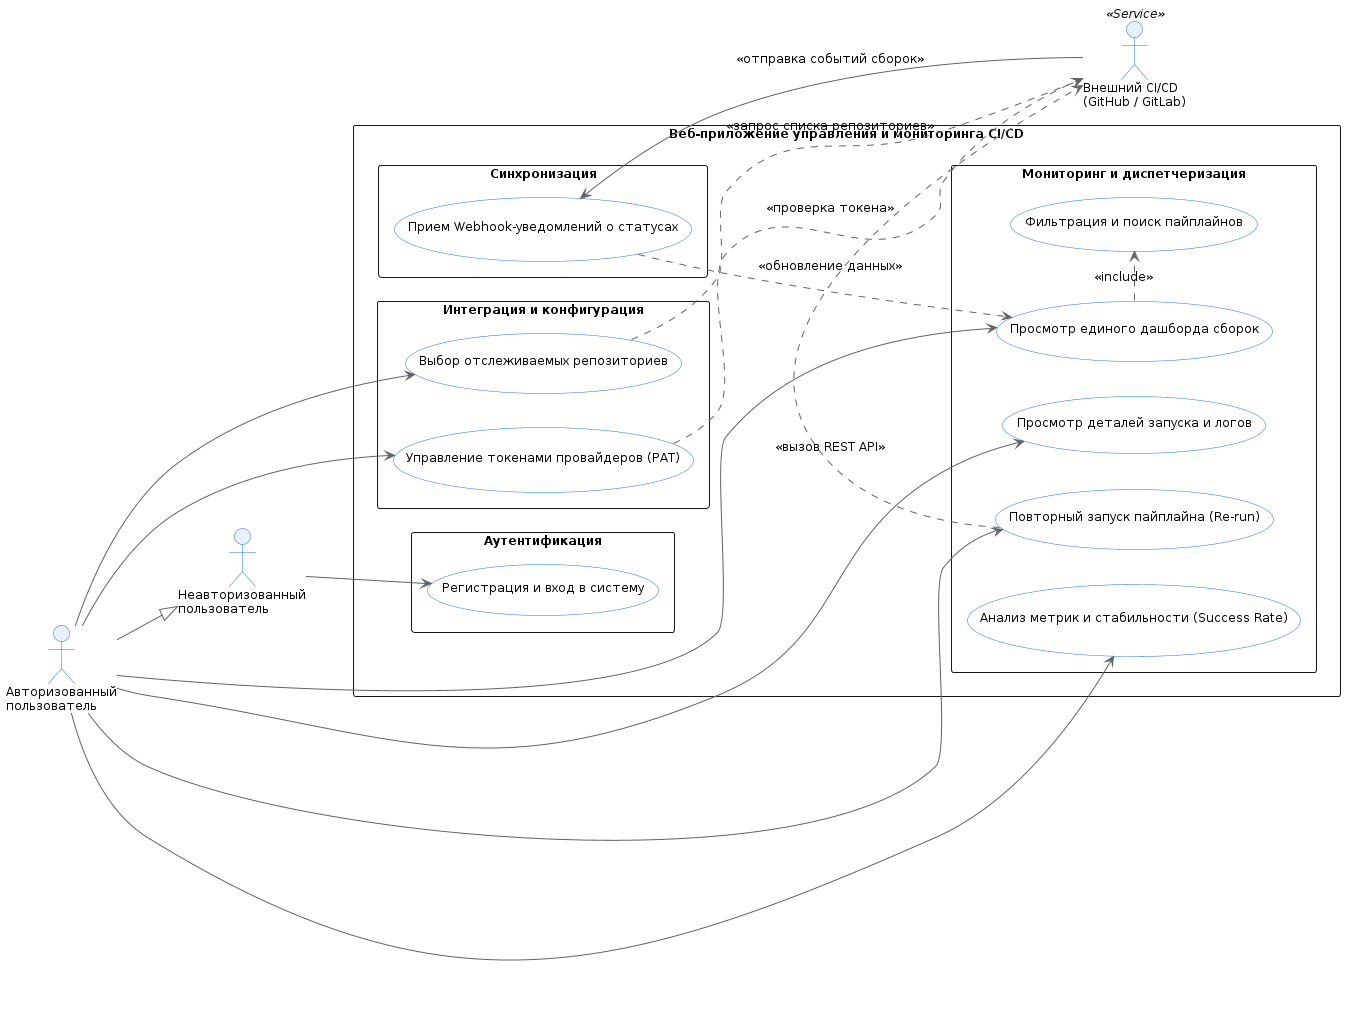
\includegraphics[width=0.85\textwidth]{images/use_case_diagram.png}
    \caption{Диаграмма вариантов использования веб-приложения}
    \label{fig:use_case}
\end{figure}

В системе выделены два действующих лица (актора):
\begin{itemize}
    \item неавторизованный пользователь (гость) --- имеет доступ только к формам входа и регистрации;
    \item авторизованный пользователь (инженер) --- имеет доступ к панели мониторинга, настройкам интеграций, управлению пайплайнами и аналитическим метрикам.
\end{itemize}

Ключевыми прецедентами являются:
\begin{itemize}
    \item управление токенами провайдеров CI/CD (GitHub PAT, GitLab Token);
    \item выбор и синхронизация отслеживаемых репозиториев;
    \item просмотр единого дашборда сборок;
    \item фильтрация и поиск пайплайнов по проектам, веткам и статусам;
    \item просмотр деталей запуска и логов выполнения сборок;
    \item диспетчеризация конвейера (повторный запуск упавших задач);
    \item анализ метрик надежности и стабильности сборок.
\end{itemize}

\subsubsection{Пользовательские истории (User Stories)}

Для детальной спецификации поведения системы разработаны пользовательские истории с критериями приемки (Acceptance Criteria), сведенные в таблицу~\ref{tab:user_stories}.

\begin{table}[H]
    \centering
    \caption{Пользовательские истории веб-приложения}
    \label{tab:user_stories}
    \small
    \resizebox{\textwidth}{!}{%
    \begin{tabular}{|l|p{4cm}|p{5cm}|p{5cm}|}
        \hline
        \textbf{ID} & \textbf{Пользовательская история} & \textbf{Критерии приемки (Given/When/Then)} & \textbf{Ценность для пользователя} \\ \hline
        US-01 & Как разработчик, я хочу подключить токен GitHub, чтобы отслеживать репозитории & \textbf{Given}: пользователь авторизован; \newline \textbf{When}: введен корректный PAT; \newline \textbf{Then}: токен зашифрован и сохранен & Безопасная интеграция без передачи основного пароля \\ \hline
        US-02 & Как инженер, я хочу видеть статусы сборок на одном экране, чтобы быстро выявлять сбои & \textbf{Given}: подключены провайдеры; \newline \textbf{When}: открыт дашборд; \newline \textbf{Then}: отображается таблица статусов & Экономия времени на переключение между системами \\ \hline
        US-03 & Как разработчик, я хочу перезапустить упавшую сборку в один клик, чтобы не заходить в GitHub & \textbf{Given}: сборка имеет статус Failed; \newline \textbf{When}: нажата кнопка «Retry»; \newline \textbf{Then}: статус сменился на Queued & Сокращение цикла исправления ошибок \\ \hline
        US-04 & Как тимлид, я хочу видеть процент успешности за неделю, чтобы оценить стабильность & \textbf{Given}: накоплена история запусков; \newline \textbf{When}: открыт раздел метрик; \newline \textbf{Then}: отображается Success Rate & Объективная оценка стабильности сборочных процессов \\ \hline
    \end{tabular}%
    }
\end{table}

\subsection{Проектирование модели данных}

Для обеспечения надежного хранения информации, транзакционной целостности и быстрого поиска по временным меткам выбрана реляционная модель данных, реализуемая в СУБД PostgreSQL.

\subsubsection{Концептуальная и логическая структура базы данных}

Модель данных спроектирована с учетом разделения сущностей на конфигурационные (пользователи, провайдеры, репозитории) и операционные (пайплайны, шаги выполнения, логи).

Связи между сущностями организованы следующим образом:
\begin{itemize}
    \item один пользователь (\texttt{users}) может сконфигурировать несколько подключений к внешним платформам (\texttt{ci\_providers}) --- связь «один-ко-многим» (1:N);
    \item каждый провайдер предоставляет доступ к множеству отслеживаемых репозиториев (\texttt{repositories}) --- связь «один-ко-многим» (1:N);
    \item репозиторий содержит историю запусков пайплайнов (\texttt{pipelines}) --- связь «один-ко-многим» (1:N);
    \item каждый запуск пайплайна детализируется последовательностью этапов выполнения (\texttt{pipeline\_steps}) --- связь «один-ко-многим» (1:N).
\end{itemize}

\subsubsection{Физическая схема базы данных}

Физическая схема разработана с соблюдением требований третьей нормальной формы (3NF). Для обеспечения информационной безопасности секретные ключи доступа (\texttt{encrypted\_token}) хранятся в зашифрованном виде с применением симметричного алгоритма Fernet.

Спецификация структуры таблиц приведена в таблицах~\ref{tab:table_users}--\ref{tab:table_steps}.

\begin{table}[H]
    \centering
    \caption{Спецификация таблицы пользователей (\texttt{users})}
    \label{tab:table_users}
    \small
    \resizebox{\textwidth}{!}{%
    \begin{tabular}{|l|l|l|p{7cm}|}
        \hline
        \textbf{Имя поля} & \textbf{Тип данных} & \textbf{Ключ} & \textbf{Описание и ограничения} \\ \hline
        \texttt{id} & INTEGER / SERIAL & PK & Уникальный идентификатор пользователя \\ \hline
        \texttt{email} & VARCHAR(255) & UNIQUE & Адрес электронной почты (логин), NOT NULL \\ \hline
        \texttt{hashed\_password} & VARCHAR(255) & — & Хеш пароля (алгоритм bcrypt), NOT NULL \\ \hline
        \texttt{full\_name} & VARCHAR(150) & — & Имя и фамилия пользователя \\ \hline
        \texttt{is\_active} & BOOLEAN & — & Флаг активности учетной записи (default: true) \\ \hline
        \texttt{created\_at} & TIMESTAMPTZ & — & Дата и время регистрации (default: NOW()) \\ \hline
    \end{tabular}%
    }
\end{table}

\begin{table}[H]
    \centering
    \caption{Спецификация таблицы провайдеров CI/CD (\texttt{ci\_providers})}
    \label{tab:table_providers}
    \small
    \resizebox{\textwidth}{!}{%
    \begin{tabular}{|l|l|l|p{7cm}|}
        \hline
        \textbf{Имя поля} & \textbf{Тип данных} & \textbf{Ключ} & \textbf{Описание и ограничения} \\ \hline
        \texttt{id} & INTEGER / SERIAL & PK & Идентификатор записи интеграции \\ \hline
        \texttt{user\_id} & INTEGER & FK & Внешний ключ на таблицу \texttt{users}, ON DELETE CASCADE \\ \hline
        \texttt{provider\_type} & VARCHAR(32) & — & Тип сервиса: \texttt{GITHUB}, \texttt{GITLAB} \\ \hline
        \texttt{name} & VARCHAR(100) & — & Пользовательское наименование подключения \\ \hline
        \texttt{api\_url} & VARCHAR(255) & — & Базовый URL API внешней платформы \\ \hline
        \texttt{encrypted\_token} & TEXT & — & Зашифрованный токен доступа (PAT), NOT NULL \\ \hline
        \texttt{is\_valid} & BOOLEAN & — & Статус валидности токена (default: true) \\ \hline
    \end{tabular}%
    }
\end{table}

\begin{table}[H]
    \centering
    \caption{Спецификация таблицы репозиториев (\texttt{repositories})}
    \label{tab:table_repos}
    \small
    \resizebox{\textwidth}{!}{%
    \begin{tabular}{|l|l|l|p{7cm}|}
        \hline
        \textbf{Имя поля} & \textbf{Тип данных} & \textbf{Ключ} & \textbf{Описание и ограничения} \\ \hline
        \texttt{id} & INTEGER / SERIAL & PK & Внутренний идентификатор репозитория \\ \hline
        \texttt{provider\_id} & INTEGER & FK & Внешний ключ на \texttt{ci\_providers}, ON DELETE CASCADE \\ \hline
        \texttt{external\_id} & VARCHAR(100) & — & Идентификатор проекта во внешней системе \\ \hline
        \texttt{full\_name} & VARCHAR(255) & — & Полное имя репозитория (\texttt{owner/repo}) \\ \hline
        \texttt{default\_branch} & VARCHAR(100) & — & Имя основной ветки (default: \texttt{main}) \\ \hline
        \texttt{web\_url} & VARCHAR(512) & — & Прямая веб-ссылка на репозиторий \\ \hline
        \texttt{is\_monitored} & BOOLEAN & — & Флаг активности мониторинга (default: true) \\ \hline
    \end{tabular}%
    }
\end{table}

\begin{table}[H]
    \centering
    \caption{Спецификация таблицы запусков пайплайнов (\texttt{pipelines})}
    \label{tab:table_pipelines}
    \small
    \resizebox{\textwidth}{!}{%
    \begin{tabular}{|l|l|l|p{7cm}|}
        \hline
        \textbf{Имя поля} & \textbf{Тип данных} & \textbf{Ключ} & \textbf{Описание и ограничения} \\ \hline
        \texttt{id} & INTEGER / SERIAL & PK & Внутренний идентификатор запуска \\ \hline
        \texttt{repository\_id} & INTEGER & FK & Внешний ключ на \texttt{repositories}, ON DELETE CASCADE \\ \hline
        \texttt{external\_run\_id} & VARCHAR(100) & — & Идентификатор прогона во внешнем API \\ \hline
        \texttt{branch} & VARCHAR(128) & — & Название целевой ветки коммита \\ \hline
        \texttt{commit\_sha} & VARCHAR(64) & — & Хеш-идентификатор коммита Git \\ \hline
        \texttt{commit\_message} & TEXT & — & Сообщение коммита \\ \hline
        \texttt{author\_name} & VARCHAR(150) & — & Автор изменений \\ \hline
        \texttt{status} & VARCHAR(32) & — & Статус: QUEUED, RUNNING, SUCCESS, FAILED \\ \hline
        \texttt{duration\_sec} & INTEGER & — & Длительность выполнения в секундах \\ \hline
        \texttt{started\_at} & TIMESTAMPTZ & — & Время запуска сборки \\ \hline
        \texttt{finished\_at} & TIMESTAMPTZ & — & Время завершения выполнения \\ \hline
    \end{tabular}%
    }
\end{table}

\begin{table}[H]
    \centering
    \caption{Спецификация таблицы стадий выполнения (\texttt{pipeline\_steps})}
    \label{tab:table_steps}
    \small
    \resizebox{\textwidth}{!}{%
    \begin{tabular}{|l|l|l|p{7cm}|}
        \hline
        \textbf{Имя поля} & \textbf{Тип данных} & \textbf{Ключ} & \textbf{Описание и ограничения} \\ \hline
        \texttt{id} & INTEGER / SERIAL & PK & Внутренний идентификатор шага \\ \hline
        \texttt{pipeline\_id} & INTEGER & FK & Внешний ключ на \texttt{pipelines}, ON DELETE CASCADE \\ \hline
        \texttt{name} & VARCHAR(150) & — & Название этапа (например, \texttt{Build}, \texttt{Test}) \\ \hline
        \texttt{stage} & VARCHAR(64) & — & Группа этапа в конвейере \\ \hline
        \texttt{status} & VARCHAR(32) & — & Статус выполнения этапа \\ \hline
        \texttt{log\_excerpt} & TEXT & — & Фрагмент вывода логов при ошибке \\ \hline
        \texttt{duration\_sec} & INTEGER & — & Длительность выполнения этапа \\ \hline
    \end{tabular}%
    }
\end{table}

Для оптимизации выполнения выборок создаются следующие индексы:
\begin{itemize}
    \item составной B-Tree индекс \texttt{idx\_pipelines\_repo\_date} по полям \texttt{(repository\_id, started\_at DESC)};
    \item индекс \texttt{idx\_pipelines\_status} по полю \texttt{status};
    \item уникальный составной индекс \texttt{uq\_repo\_external\_id} на поля \texttt{(provider\_id, external\_id)}.
\end{itemize}

\subsection{Разработка макетов страниц (Wireframe)}

Пользовательский интерфейс проектируется в соответствии с концепцией Single Page Application (SPA). Главной задачей интерфейса является обеспечение высокой информативности без визуальной перегруженности, позволяя оператору за минимальное время оценить статус инфраструктуры.

В системе выделены 4 ключевых экрана:
\begin{enumerate}
    \item Экран аутентификации (\texttt{/login}). Компактная форма по центру экрана, содержащая поля ввода Email и пароля, валидацию ошибок ввода и кнопку входа.
    \item Главная панель мониторинга (\texttt{/dashboard}). Основное рабочее пространство. В верхней части расположены карточки сводных показателей, под ними находится панель фильтрации, а центральную часть занимает таблица сборок с кнопками ручного перезапуска.
    \item Экран деталей запуска и логов (\texttt{/pipelines/:id}). Отображает последовательность стадий конвейера и окно терминала с моноширинным шрифтом для вывода логов ошибок.
    \item Экран настроек интеграций (\texttt{/settings/integrations}). Форма для добавления новых подключений к Git-платформам и переключатели отслеживаемых репозиториев.
\end{enumerate}

Схематический макет ключевого экрана мониторинга сборок (Wireframe) приведен на рисунке~\ref{fig:wireframe_dashboard}.

\begin{figure}[H]
    \centering
    \footnotesize
    \begin{verbatim}
+----------------------------------------------------------------+
| CI/CD Monitor & Dispatcher   [Dashboard] [Settings]    (User)  |
+----------------------------------------------------------------+
| [Total: 1420]   [Success: 94%]   [Running: 3]   [Failed: 12]   |
+----------------------------------------------------------------+
| Filters: [All Repos v]      [Branch: main v]   [Status: All v] |
+----------------------------------------------------------------+
| Repository    Branch    Commit / Author   Duration  Status     |
+----------------------------------------------------------------+
| auth-service  main      f8a12c Fix JWT    1m 45s    [ SUCCESS ]|
| billing-api   develop   90c21b Add Stripe 3m 12s    [ FAILED  ]|
| frontend-web  feature-x e711a0 UI Update  2m 04s    [ RUNNING ]|
+----------------------------------------------------------------+
| Showing 1-3 of 84 runs                  < Prev [1] 2 3 Next >  |
+----------------------------------------------------------------+
    \end{verbatim}
    \caption{Схематический макет главного экрана мониторинга сборок (Wireframe)}
    \label{fig:wireframe_dashboard}
\end{figure}

Спроектированная архитектура интерфейса и структуры данных обеспечивает выполнение всех функциональных требований, определенных в аналитическом разделе, и формирует полную спецификацию для этапа программной реализации.